\section{Materials}
\label{sec:materials}

This section describes the EPIC-KITCHENS-100 dataset, the empirical exploration that informed our preprocessing decisions, and the pre-trained checkpoints, hardware and software stack that supported the three approaches.

\subsection{Dataset and empirical exploration}
\label{sec:materials:data}

\begin{figure}[t]
    \centering
    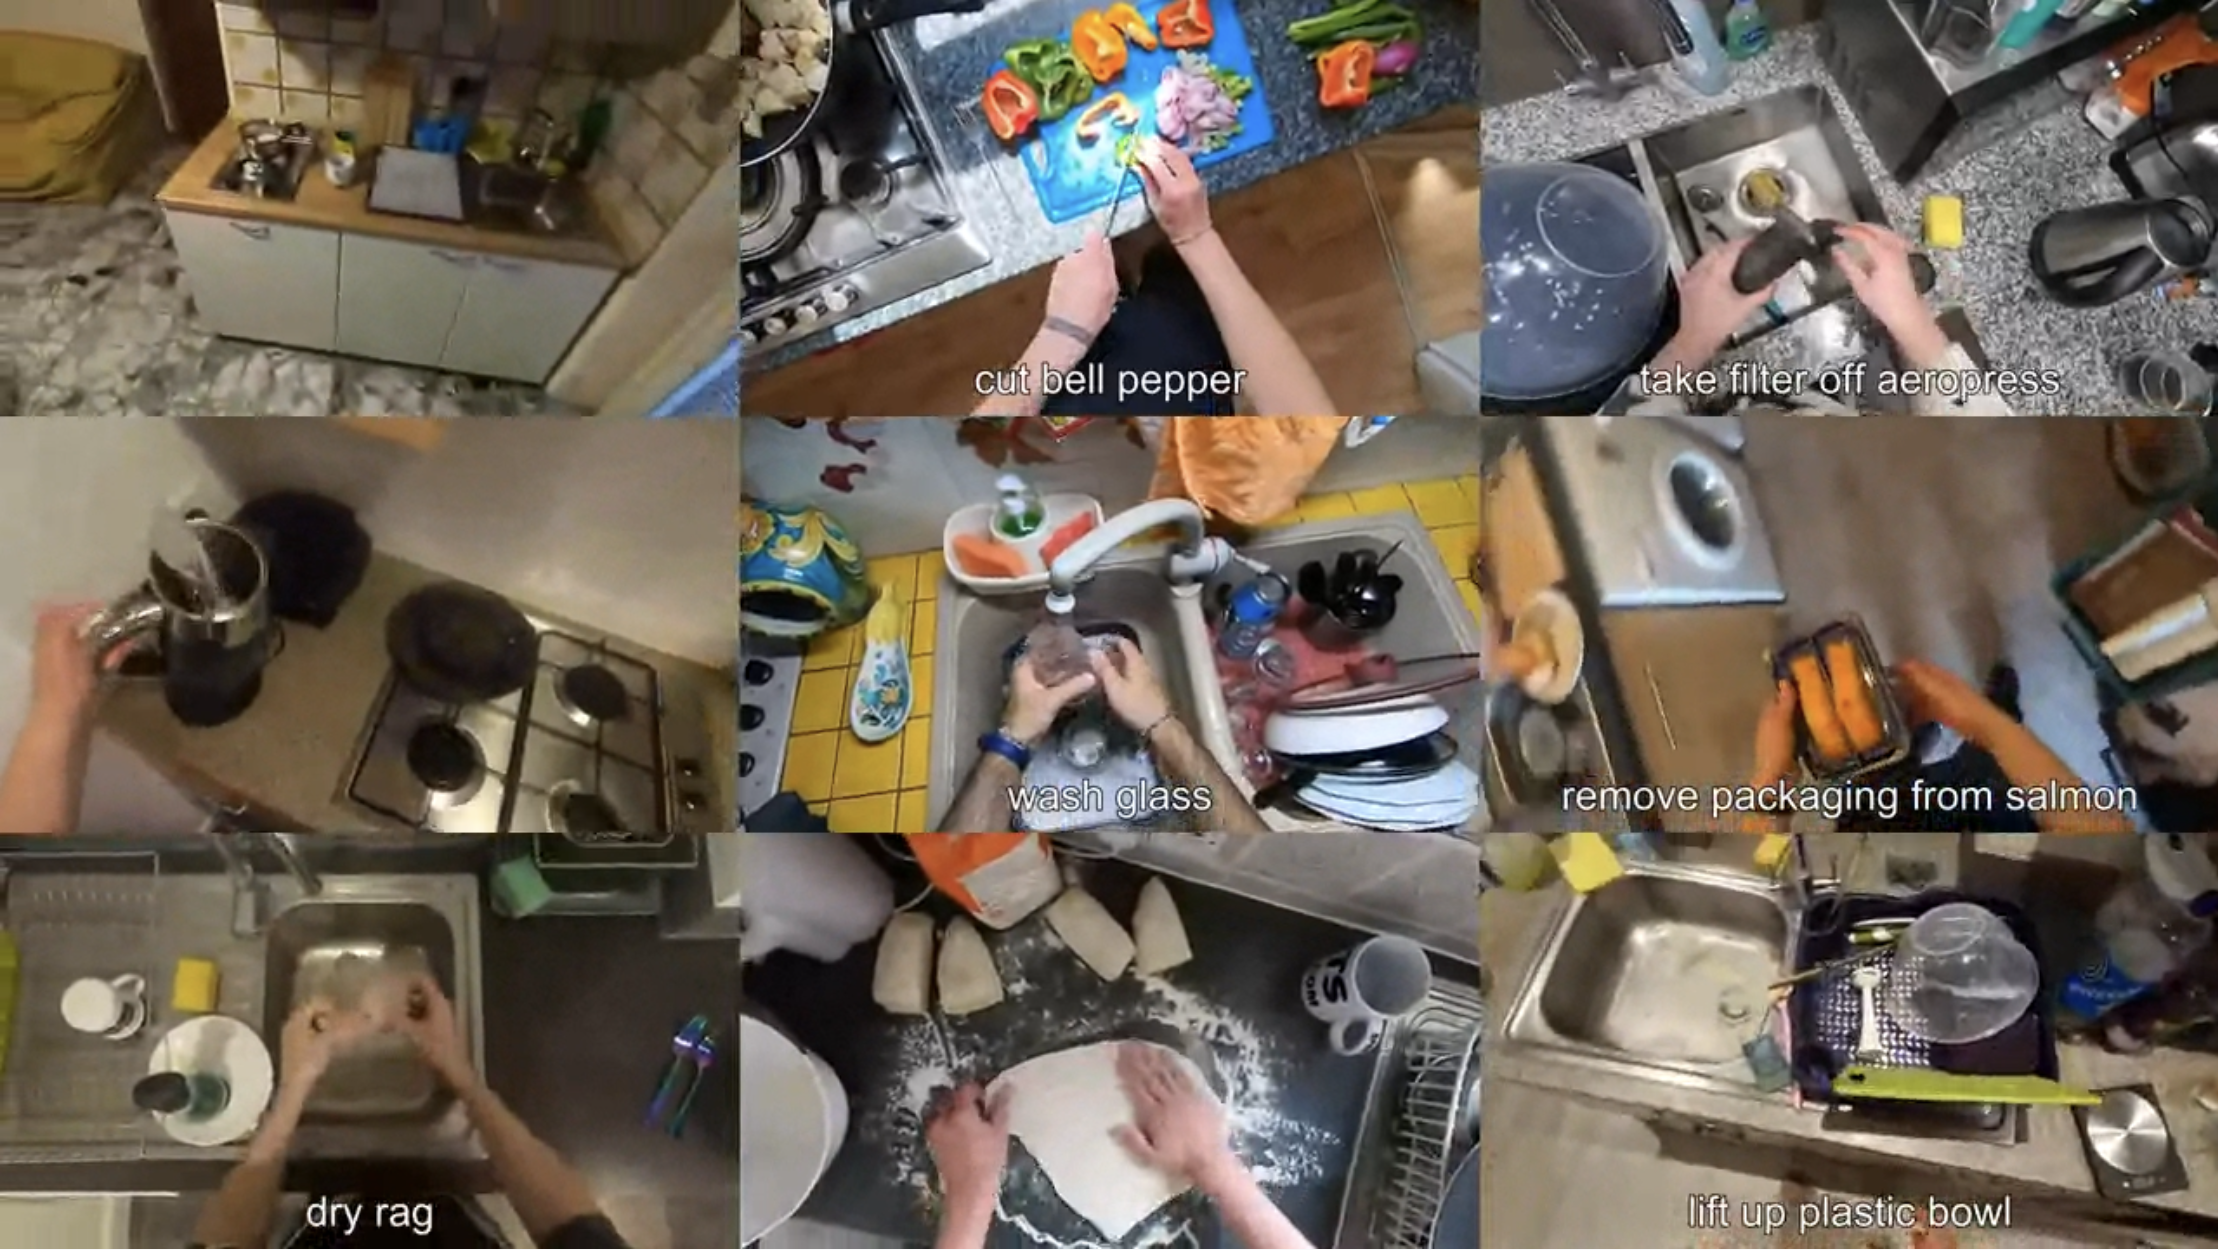
\includegraphics[width=\columnwidth]{images/collage.png}
    \caption{Qualitative overview of EPIC-KITCHENS-100 with multiple example frames illustrating different kitchens, viewpoints and activities.}
    \label{fig:dataset_collage}
\end{figure}

We use the EPIC-KITCHENS-100 dataset, focusing on the Multi-Instance Retrieval (MIR) challenge. The corpus comprises trimmed egocentric action segments paired with English narrations, recorded with head-mounted cameras in 45 kitchens and totaling 100 hours of Full-HD video. This encompasses around 20\,M frames distributed in 700 variable-length sequences with 97 verb classes and 300 noun classes~\cite{damen2022rescaling}. The retrieval split releases $67{,}217$ training segments and $9{,}668$ test segments paired with $3{,}842$ unique narrations on the test side. Ground-truth relevance is provided as the soft-label matrix released by Wray et al.~\cite{wray2021semantic} alongside the dataset. The \emph{test} relevance matrix is held out by the organizers and available exclusively through the Codabench grader, restricting offline metric computation to the public training and validation splits. Figure~\ref{fig:dataset_collage} illustrates the visual diversity of the corpus.

The retrieval annotations define each training segment from its start and stop frames and the recording frame rate, $\texttt{dur} = (\texttt{stop\_frame} - \texttt{start\_frame} + 1)/\texttt{fps}$. Across the $67{,}217$ training segments the mean duration is $3.18$\,s (median $1.6$\,s), with a long tail of extended actions reaching $\sim 297$\,s. This variability motivates evaluating a longer-clip test-time augmentation in Section~\ref{sec:methods:avion}, where the default 8-frame clips are complemented with 32-frame clips.

\subsection{Pre-trained checkpoints, hardware and software}
\label{sec:materials:stack}

All three configurations reuse publicly released checkpoints. Configurations~1 and~2 operate on pre-extracted features and were executed on a single NVIDIA T4 (16\,GB), using the JPoSE and MMEN encoders distributed by Wray et al.~\cite{wray2019jpose} together with the MI-MM checkpoint and S3D-HowTo100M features released alongside MIL-NCE~\cite{miech2020milnce}. Configuration~3 fine-tunes a ViT-L/14 backbone from the AVION pre-train checkpoint of Zhao and Kr\"ahenb\"uhl~\cite{zhao2023avion} on a single NVIDIA A100 (40\,GB), using gradient checkpointing, the \texttt{use-fast-conv1} optimization of AVION, FlashAttention~\cite{dao2022flashattention} when available, AdamW~\cite{loshchilov2019adamw}, a base learning rate of $2\times 10^{-5}$ and batch size $48$. This configuration also requires staging $\approx 720$\,GB of EK-100 video chunks (320p, 15\,s, 30\,fps, libx264) on persistent storage, together with the EK-100 retrieval annotations and the public training relevancy matrix~\cite{wray2021semantic}. The implementation is built on PyTorch 2.4.1 (CUDA 12.1) with standard vision--language components and \texttt{decord} for video I/O. The SMS-Loss code is a patched fork of the public release~\cite{wang2024smsloss_repo,wang2024symmetricmultisimilaritylossepickitchens100} that fixes a small number of bugs preventing stable end-to-end runs on EK-100.
